\section{Mô hình kiến trúc ứng dụng iOS}
Lựa chọn mô hình kiến trúc phù hợp là quyết định quan trọng ảnh hưởng đến khả năng bảo trì, mở rộng và kiểm thử của ứng dụng. Dưới đây là các mô hình phổ biến trong phát triển iOS:

\begin{figure}[H] 
    \centering
    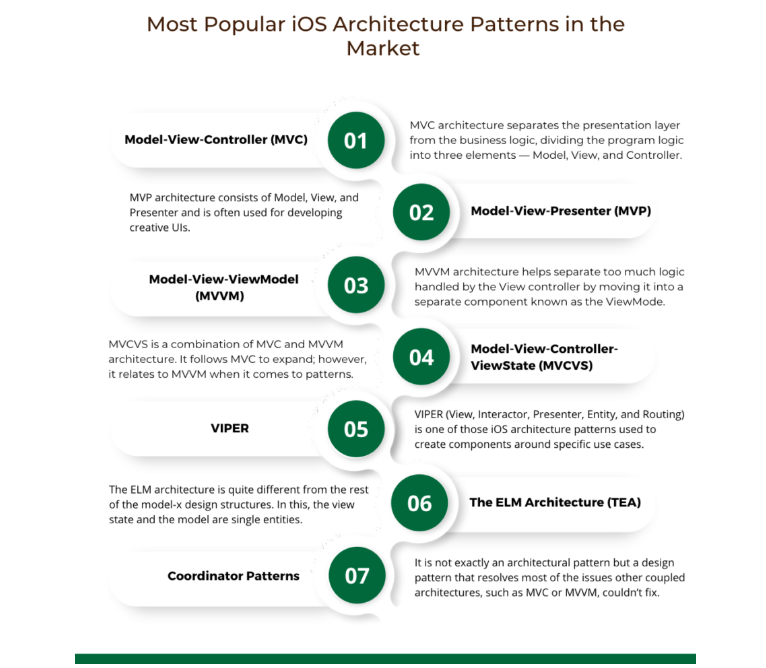
\includegraphics[width=0.8\textwidth]{images/mohinhkientrucios.png}
     \caption{Một số mô hình kiến trúc IOS}
    \label{fig:mohinhkientrucios}
\end{figure}
    \subsection{Model-View-Controller(MVC)}
    MVC (Model-View-Controller) là một trong những mô hình kiến trúc truyền thống được Apple khuyến nghị sử dụng trong quá khứ để xây dựng ứng dụng iOS.\\
    \vspace{1em}
    \textbf{Thành phần:}
    \begin{description}
      \item[Model:] Quản lý dữ liệu và logic nghiệp vụ.
      \item[View:] Hiển thị giao diện người dùng và phản hồi tương tác.
      \item[Controller:] Trung gian giữa Model và View, xử lý logic điều khiển.
    \end{description}
    
    \vspace{1em}
    \textbf{Ưu điểm:}
    \begin{description}
      \item[•] Là một trong những mẫu kiến trúc ứng dụng iOS phổ biến nhất, được sử dụng trong cả phát triển ứng dụng và web.
      \item[•] Dễ dàng phân tách trách nhiệm giữa máy chủ và máy khách.
      \item[•] Phù hợp cho các ứng dụng nhỏ và đơn giản.
    \end{description}
    
    \vspace{1em}
    \textbf{Nhược điểm:}
    \begin{description}
      \item[•] ``Massive View Controller'' – Controller thường trở nên quá lớn và phức tạp.
      \item[•] Khó khăn trong việc kiểm thử.
      \item[•] Sự phụ thuộc chặt chẽ giữa các thành phần.
    \end{description}
    \subsection{Mô hình MVP trong iOS}

    MVP (Model-View-Presenter) là một biến thể của MVC, tập trung vào việc tách riêng phần hiển thị (View) và logic điều khiển (Presenter), giúp tăng khả năng kiểm thử và tái sử dụng.
    
    \vspace{1em}
    \textbf{Thành phần:}
    \begin{description}
      \item[Model:] Tương tự như trong MVC.
      \item[View:] Giao diện thụ động, chỉ hiển thị dữ liệu.
      \item[Presenter:] Xử lý logic nghiệp vụ và cập nhật View.
    \end{description}
    
    \vspace{1em}
    \textbf{Ưu điểm:}
    \begin{description}
      \item[•] View hoàn toàn thụ động, dễ kiểm thử.
      \item[•] Xác minh chức năng chính xác của từng thành phần trở nên dễ tiếp cận hơn trong MVP.
      \item[•] Presenter có thể được tái sử dụng với các View khác nhau.
    \end{description}
    
    \vspace{1em}
    \textbf{Nhược điểm:}
    \begin{description}
      \item[•] Cần nhiều mã \textit{boilerplate}.
      \item[•] Presenter có thể trở nên lớn và phức tạp.
      \item[•] Không phổ biến bằng MVVM trong cộng đồng iOS.
    \end{description}
    

    \subsection{Mô hình MVVM trong iOS}

    MVVM (Model-View-ViewModel) là mô hình kiến trúc hiện đại được sử dụng phổ biến trong phát triển ứng dụng iOS, đặc biệt khi kết hợp với các framework reactive như Combine hoặc RxSwift.

    \vspace{1em}
    \textbf{Thành phần:}
    \begin{description}
    \item[Model:] Tương tự như trong MVC.
    \item[View:] Bao gồm \textbf{UIView} và \textbf{UIViewController}.
    \item[ViewModel:] Chuẩn bị dữ liệu từ Model để View hiển thị và xử lý logic.
    \end{description}

    \vspace{1em}
    \textbf{Bốn nguyên tắc trong MVVM:}
    \begin{description}
        \item[The Simplicity Principle (Nguyên tắc đơn giản):] Mỗi View chỉ nên có một ViewModel tương ứng. Mỗi ViewModel chỉ phục vụ một View duy nhất.
        \item[The Blendability Principle (Nguyên tắc hòa trộn):] ViewModel cần hỗ trợ khả năng hòa trộn biểu thức để tối ưu hóa UI.
        \item[The Designability Principle (Nguyên tắc thiết kế):] ViewModel phải cung cấp dữ liệu có thể dùng tại thời điểm thiết kế (design-time).
        \item[The Testability Principle (Nguyên tắc kiểm thử):] Cả Model và ViewModel đều phải có khả năng kiểm thử độc lập.
    \end{description}

    \vspace{1em}
    \textbf{Ưu điểm:}
    \begin{description}
    \item[•] Tách biệt rõ ràng các thành phần.
    \item[•] Dễ dàng kiểm thử (đặc biệt là ViewModel).
    \item[•] Giảm kích thước và trách nhiệm của ViewController.
    \item[•] Hỗ trợ binding dữ liệu giữa View và ViewModel.
    \end{description}

    \vspace{1em}
    \textbf{Nhược điểm:}
    \begin{description}
    \item[•] Phức tạp hơn so với MVC.
    \item[•] Có thể dẫn đến ``Massive ViewModel'' nếu không được tổ chức tốt.
    \item[•] Yêu cầu cơ chế binding (thủ công hoặc sử dụng thư viện reactive).
    \end{description}
    \subsection{MVCVS (Model-View-Controller-ViewState)}

    MVCVS bằng cách nào đó là sự kết hợp giữa hai kiến trúc MVC và MVVM. Nó giúp tách biệt rõ ràng giữa \textbf{Model}, \textbf{View}, \textbf{Controller}, và \textbf{View State}.
    
    \textbf{Các giai đoạn hoạt động của MVCVS:}
    \begin{description}
      \item[MVCVS Initialization:] Ở giai đoạn này, View Controller phải tuân theo Model và View State.
      \item[MVCVS Model Updates:] Nếu có bất kỳ thay đổi nào xảy ra, View Controller sẽ cập nhật Document Model và View State.
      \item[MVCVS View Changes:] View State phân tích Document View Model và View State. Sau đó, nó thực hiện các thay đổi đối với View dựa trên các quan sát.
      \item[MVCVS View State:] View Controller và View State được tách biệt. View State chịu trách nhiệm cập nhật và lắng nghe các thay đổi trong View.
      \item[MVCVS Testability:] Có thể kiểm tra logic của View Model và Document Model một cách riêng biệt, giúp việc kiểm thử hiệu quả hơn so với mô hình MVC.
    \end{description}
    
    \textbf{Ưu điểm:}
    \begin{itemize}
      \item Là mẫu kiến trúc có khả năng quản lý và hiệu quả cao.
      \item Dễ dàng kiểm tra riêng biệt các thành phần nhờ các bài kiểm tra tích hợp.
    \end{itemize}
    
    \textbf{Nhược điểm:}
    \begin{itemize}
      \item Độ phức tạp cao.
      \item Khó tiếp cận đối với người mới.
    \end{itemize}
    
    \subsection{VIPER}

    Là một trong những mẫu kiến trúc iOS được biết đến với cấu trúc clean. Đây là lựa chọn phù hợp khi cần tạo các thành phần xoay quanh các trường hợp sử dụng cụ thể.
    
    \textbf{Các thành phần trong VIPER:}
    \begin{description}
      \item[View:] Giao diện người dùng.
      \item[Interactor:] Xử lý logic nghiệp vụ.
      \item[Presenter:] Điều phối giữa View và Interactor.
      \item[Entity:] Mô hình dữ liệu.
      \item[Routing:] Điều hướng giữa các màn hình.
    \end{description}
    
    \textbf{Ưu điểm:}
    \begin{itemize}
      \item Kiến trúc dễ quản lý, phù hợp với nhóm phát triển lớn.
      \item Tăng khả năng tái sử dụng mã nguồn.
      \item UI được xác định rõ ràng và dễ kiểm soát.
      \item Mã được phân tách giúp kiểm thử dễ dàng.
      \item Giảm thiểu xung đột hợp nhất mã.
    \end{itemize}
    
    \textbf{Nhược điểm:}
    \begin{itemize}
      \item Cấu trúc phức tạp đối với ứng dụng nhỏ.
      \item Tốn thời gian để làm quen.
      \item Nhiều lớp trung gian có thể làm giảm hiệu suất.
    \end{itemize}
    
    \subsection{The Elm Architecture (TEA)}
    
    TEA là một mô hình kiến trúc mới trong iOS, khá khác biệt so với các cấu trúc Model-X truyền thống. Trạng thái giao diện và mô hình được hợp nhất thành một thực thể duy nhất. Mọi cập nhật được gửi đến thực thể này dưới dạng \textbf{messages} và xử lý thông qua \textbf{reducers}.
    
    Dòng sự kiện trong TEA là một chiều (unidirectional), tương tự như Flux hoặc Redux.
    
    \textbf{Ưu điểm:}
    \begin{itemize}
      \item View có thể được mô tả như các hàm thuần túy (pure functions).
      \item One-way binding từ Model đến View giúp dễ kiểm soát.
    \end{itemize}
    
    \textbf{Nhược điểm:}
    \begin{itemize}
      \item Tăng độ phức tạp trong các ứng dụng lớn.
      \item Không phù hợp với mọi loại ứng dụng.
    \end{itemize}
    
    \subsection{Coordinator Pattern}
    
    Mặc dù không phải là một mẫu kiến trúc chính thức, Coordinator là một \textbf{design pattern} giúp giải quyết các vấn đề điều hướng mà MVC hoặc MVVM không xử lý tốt.
    
    Coordinator chịu trách nhiệm tạo và giữ tham chiếu đến ViewController hiện tại. Nó thực hiện việc điều hướng, ví dụ: hiển thị màn hình mới hoặc đẩy ViewController vào Navigation Controller.
    
    \textbf{Ưu điểm:}
    \begin{itemize}
      \item Tách riêng logic điều hướng, giúp mã dễ bảo trì.
      \item Tăng tính linh hoạt trong chuyển đổi giữa các màn hình.
    \end{itemize}
    
    \textbf{Nhược điểm:}
    \begin{itemize}
      \item Làm tăng độ phức tạp khi triển khai.
      \item Cần thay đổi cách tiếp cận luồng dữ liệu.
      \item Không cần thiết cho các ứng dụng nhỏ.
    \end{itemize}
    